\documentclass[onecolumn]{article}
\usepackage{fullpage}
\usepackage[utf8]{inputenc}
\usepackage[spanish]{babel}
\usepackage{amsmath}
\usepackage{amsfonts}
\usepackage{amssymb}
\usepackage{graphicx}
\usepackage{url}
\usepackage{hyperref}

\usepackage[T1]{fontenc}
\renewcommand*\familydefault{\sfdefault} %% Only if the base font of the document is to be sans serif

\usepackage{listings}
\lstdefinelanguage{VHDL}{
   morekeywords={
     library,use,all,entity,is,port,in,out,end,architecture,of,
     begin,and
   },
   morecomment=[l]--
}
 
\usepackage{xcolor}
\colorlet{keyword}{blue!100!black!80}
\colorlet{comment}{green!90!black!90}
\lstdefinestyle{vhdl}{
   language     = VHDL,
   basicstyle   = \ttfamily,
   keywordstyle = \color{keyword}\bfseries,
   commentstyle = \color{comment}
}
 


\begin{document}

\title{Plantilla \LaTeX - Laboratorios Organización de Computadores}
\author{Autor 1 - Autor 2 - Autor 3\\
Pontificia Universidad Javeriana\\
Organización de Computadores
}
\date{\today}

\maketitle

\begin{abstract}
Texto de resumen. Texto de resumen. Texto de resumen. Texto de resumen. Texto de resumen. Texto de resumen. Texto de resumen. Texto de resumen. Texto de resumen. Texto de resumen. Texto de resumen. Texto de resumen. Texto de resumen. Texto de resumen. Texto de resumen. Texto de resumen. Texto de resumen. Texto de resumen. Texto de resumen. Texto de resumen. Texto de resumen. Texto de resumen. Texto de resumen.
\end{abstract}

\section{Sección cero}


%///////////////////////////////////////////
\section{Sección Primera}
%///////////////////////////////////////////

Contenido de la sección. Contenido de la sección. Contenido de la sección. Contenido de la sección. Contenido de la sección. Contenido de la sección. Contenido de la sección. Contenido de la sección. Contenido de la sección. Contenido de la sección. Contenido de la sección. Contenido de la sección. Contenido de la sección. Contenido de la sección. Contenido de la sección. Contenido de la sección. Contenido de la sección. Contenido de la sección. Contenido de la sección. 

Este es un ejemplo de como referenciar la Figura \ref{fig:pcb}. Si no es una figura propia, se debe referenciar a la respectiva fuente \footnote{Tomado de \url{http://www.jps-pcb.com/blog/3-main-failure-modes-of-electronics.html}}.

\begin{figure}[ht!]
	\centering
	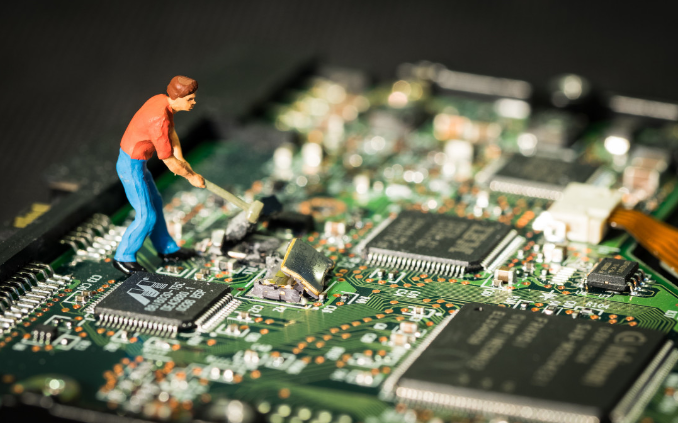
\includegraphics[width=3in]{pcb.png}
	\caption{Un ejemplo para incluir una figura. }
	\label{fig:pcb}
\end{figure}


%///////////////////////////////////////////
\section{Sección Segunda}
%///////////////////////////////////////////

Ejemplo de como incluir código en VHDL y referencia el código fuente \ref{lst:list1}:

\begin{lstlisting}[caption={Ejemplo de como incluir código fuente.}\label{lst:list1},style=vhdl] 
library IEEE;
use IEEE.STD_LOGIC_1164.ALL;
use IEEE.STD_LOGIC_UNSIGNED.ALL;

entity up_dn_counter_top is
    Port ( CLK : in  STD_LOGIC;     -- input clock
           LED : out  STD_LOGIC_VECTOR (7 downto 0);
           DIR : in  STD_LOGIC);    -- direction of counter (up or down)
end up_dn_counter_top;

architecture Behavioral of up_dn_counter_top is
    signal count   : STD_LOGIC_VECTOR (7 downto 0) := X"00";
begin    
    process (CLK, DIR)
    begin
        if (CLK'Event and CLK = '1') then
            if (DIR = '1') then
                count <= count + '1';   -- counting up
            elsif (DIR = '0') then
                count <= count - '1';   -- counting down
            end if;
        end if;
    end process;
    -- display count on LEDs
    LED <= not count;
end Behavioral;

\end{lstlisting}


%///////////////////////////////////////////
\section*{Referencias}
%///////////////////////////////////////////

\begin{itemize}
	\item Referencia 1. Libro. Editorial. Año.
	\item Referencia 2. Libro. Editorial. Año.
\end{itemize}


\end{document}


